%!TEX root = ../all.tex
% =============================================================================
%  CADET - The Chromatography Analysis and Design Toolkit
%  
%  Copyright © 2008-2020: The CADET Authors
%            Please see the AUTHORS and CONTRIBUTORS file.
%  
%  All rights reserved. This program and the accompanying materials
%  are made available under the terms of the GNU Public License v3.0 (or, at
%  your option, any later version) which accompanies this distribution, and
%  is available at http://www.gnu.org/licenses/gpl.html
% =============================================================================

\chapter{Models}

%\section{Terms and physical phenomena}
%
%\begin{description}
%	\item[Convective transport] Transport of the solute molecules by convection (i.e., movement with the flow of the liquid).
%	\item[Dispersion] Band broadening effect caused by the non-ideal flow due to the packed bed.
%	\item[Diffusion] Brownian motion of the molecules.
%	\item[Film diffusion] 
%\end{description}

\section{Network of unit operation models}\label{sec:MUOPNetwork}

Unit operation models can be composed into a network \index{Model!Network}\index{Network} or graph, in which a node represents a unit operation and an edge denotes a connection between two unit operations.
When utilized to full extent, this allows the simulation of complicated setups and processes (e.g., SMB, MCSGP).
A more simple use case is the addition of plug flows and stirred tanks up- and downstream of a column in order to account for dead volume and additional dispersion from the tubing.

In a network, outlet ports of unit operations can be connected to any number of inlet ports of unit operations.
Even direct cycles, where an outlet port of a unit operation is connected to its own inlet, are possible.
A unit operation does not have to possess both inlet and outlet, but it has to have at least one of them.
Pseudo unit operations such as inlet and outlet serve as sources and sinks for the network.
However, the latter is not strictly required as any terminal node (i.e., a unit operation that possesses an outlet but does not have an outgoing connection) serves as a sink.

Each connection between two unit operation ports (i.e., an edge in the graph) is equipped with a volumetric flow rate that determines the mass flow from source to target port.
These flow rates are used to determine the weight of the different incoming feeds at a unit operation's inlet port.
Some unit operations can infer their internal flow rate (e.g., interstitial velocity) from their total incoming volumetric flow rate.
In general, the mass balance at a unit operation has to be closed, except for unit operations that act as source or sink in the network and variable volume units (e.g., stirred tanks).

The network of unit operations uses ``connection''-variables $c_{\text{con}}$ to connect the different unit operation ports with each other.
The inlet port variables $c_{\text{in},n,k}$ of unit operation $n$ are attached to $c_{\text{con},n}$ via 
\begin{align}
	c_{\text{in},n,k,i} &= c_{\text{con},n,k,i}, \qquad k = 1, \dots, N_{\text{port},\text{in},n},\quad i = 1, \dots, N_{\text{comp},n}. \label{eq:NetworkInletConnection}
\end{align}
While $N_{\text{port},\text{in},n}$ denotes the number of inlet ports of unit operation $n$, the number of outlet ports is given by $N_{\text{port},\text{out},n}$.
The connection variables $c_{\text{con},n,k,i}$ collect all inflows of component $i$ into port $k$ of unit operation $n$:
\begin{align}
	c_{\text{con},n,k,i} &= \frac{\sum_{m=1}^{N_{\text{units}}} \sum_{\ell = 1}^{N_{\text{port},\text{out},n}} \sum_{j = 1}^{N_{\text{comp},m}} S_{(n,k,i),(m,\ell,j)} Q_{m,\ell} c_{\text{out},m,\ell,j}}{\sum_{m=1}^{N_{\text{units}}} \sum_{\ell=1}^{N_{\text{port},\text{out},m}} \hat{S}_{(n,k),(m,\ell)} Q_{m,\ell} }, \label{eq:NetworkConnection}
\end{align}
where $Q_{m,\ell}$ denotes the volumetric flow rate from outlet port $\ell$ of unit operation $m$, $S_{(n,k,i),(m,\ell,j)} \in \{0, 1\}$ is a connection matrix indicating whether component $i$ at outlet port $k$ of unit operation $n$ is connected to component $j$ at inlet port $\ell$ of unit operation $m$, and $\hat{S}_{(n,k),(m,\ell)} \in \{0, 1\}$ is another connection matrix indicating whether outlet port $k$ of unit operation $n$ is connected to inlet port $\ell$ of unit operation $m$, that is
\begin{align*}
	\hat{S}_{(n,k),(m,\ell)} = \begin{cases}
		1 & \text{if } \sum_{i = 1}^{N_{\text{comp},n}} \sum_{j = 1}^{N_{\text{comp},m}} S_{(n,k,i),(m,\ell,j)} \geq 1, \\
		0 & \text{otherwise}.
	\end{cases}
\end{align*}

Note that for each unit operation the number of inlet ports may be different from the number of outlet ports.
Hence, the mass balance of a single unit operation is taken with respect to all its ports combined.

\paragraph{Specification of network connections}
\phantomsection\label{par:MUOPNetworkConfig}

The connections \index{Network!Connectivity} between the different unit operations in the network are specified by a table.
There are two table formats:
\begin{itemize}
	\item The long format includes seven columns.
	The first two columns specify source and destination unit operation id.
	The next two columns give source and destination port indices.
	Source and destination component indices are given by the following two columns.
	Finally, the seventh column specifies the volumetric flow rate of this connection.
	\item The short format includes five columns.
	The first two columns specify source and destination unit operation id.
	Source and destination component indices are given by the following two columns.
	Finally, the fifth column specifies the volumetric flow rate of this connection.
	Here, the omitted port indices default to $-1$, which connects all ports of the source unit operation to the corresponding ports of the target. 
\end{itemize}
By default, the short format is used (i.e., a table with five columns is expected).
However, if a unit operation with multiple ports is present, a table with seven columns is required.
The default format can be overruled by setting a field (see Table~\ref{tab:FFModelConnectionSwitch}).

With this setup, it is possible to connect single components of unit operations with each other yielding a maximum in flexibility.
However, the predominant case is to connect all components of the source unit operations with their respective counterparts in the destination unit.
This can easily be done by setting both component indices to $-1$ instead of writing a separate row for each component of the connection.
The same setting (i.e., setting both port indices to $-1$) can be used to connect all ports of one unit operation with all corresponding ports of another one.

Note that in case of multiple rows for one connection between two unit operation ports (e.g., in case of separate component connections) the flow rate of the first row of that connection is used and all following flow rates are ignored.
Consequently, there can only be one flow rate for a connection between two unit operations regardless of which components are connected.

The connection table is expected in row-major storage format (i.e., the rows are appended to one long array).
See Table~\ref{tab:FFModelConnectionSwitch}.

\paragraph{Valve switches}
\phantomsection\label{par:MUOPNetworkValveSwitches}

The connectivity of the network can only change on a discontinuous section transition.
Such a transition with changing connectivity is referred to as valve switch and the connectivity itself as valve configuration. \index{Network!Valve switch}

A list of valve configurations with at least one entry is required.
Each valve configuration consists of a network connectivity table as described in Section~\ref{par:MUOPNetworkConfig} and a section index.
The latter denotes the section in which the connectivity table becomes active.
Hence, the one required (i.e., the first) entry must have a section index of $0$ denoting the initial connectivity.

Note that the section index has to be monotonically increasing throughout the list of valve configurations.
See Tables~\ref{tab:FFModelSystemConnections} and \ref{tab:FFModelConnectionSwitch}.

\paragraph{Dynamic flow rates}
\phantomsection\label{par:MUOPNetworkDynamicFlowRates}

The volumetric flow rates may vary over time while the valve configuration is active.
The rates are assumed to be cubic polynomials,
\begin{align*}
	Q = Q_0 + Q_1(t - t_s) + Q_2(t-t_s)^2 + Q_3(t-t_s)^3,
\end{align*}
where $t_s$ is the beginning of the time section that triggers the valve switch.

Note that the denominator in Eq.~\ref{eq:NetworkConnection} must always be positive.
That is, the flow rate coefficients have to be chosen such that the flow into every connected inlet port is strictly positive at all times.

\paragraph{Solution of the linear systems}
\phantomsection\label{par:MUOPNetworkLinearSolver}

Each time step in the simulation requires the solution of a nonlinear system Eq.~\eqref{eq:BDFNonlinSystem} (see Sec.~\ref{sec:SimTimeIntegration}).
The nonlinear problem is solved by a Newton iteration, which, in turn, requires the solution of a linear system that essentially consists of the Jacobians of the unit operations and some coupling matrices from Eqs.~\eqref{eq:NetworkInletConnection} and \eqref{eq:NetworkConnection}.

These linear systems are either solved in parallel or sequentially.
The parallel method first solves each unit operation (in parallel) to compute the solution at its outlet.
Using these values, the inlets are adjusted and the unit operations are solved again.
This is iterated until the system is fully solved.

In contrast, the sequential method first determines an ordering of the unit operations such that each unit only receives inflow from the previous units in the ordering.
Such an ordering requires an acyclic graph of unit operations.
Finally, the linear system is solved by solving the unit operations in the ordering determined above.
Before a unit is solved, its inlet is calculated from the outlets of the previously solved units.
This means, the system is solved from system inlets to system outlets.

The parallel method works regardless of the network topology (i.e., cycles in the graph), but requires to solve each unit operation at least twice.
The sequential method solvs each unit exactly once, but is restricted to acyclic networks and works best for small graphs.
By default, \CADET{} uses a heuristic to select an appropriate solution method.
This default can be overridden by a flag (see Table~\ref{tab:FFModelSolver}).

The solution method is selected for each valve switch individually.
If some network configurations contain cycles, the parallel method is chosen for them regardless of the method used for the other configurations.

\section{Unit operation models}

\phantomsection\label{par:MFeatureMatrix}

A short comparison of the most prominent unit operation model features is given in Table~\ref{tab:MFeatureMatrix}.

\begin{table}[!ht]
\centering
\begin{tabu}to \linewidth[m]{X>{\centering\arraybackslash}p{1.6cm}>{\centering\arraybackslash}p{1.6cm}>{\centering\arraybackslash}p{1.6cm}>{\centering\arraybackslash}p{1.6cm}>{\centering\arraybackslash}p{1.6cm}} \toprule
\rowfont[c]\normalfont Unit operation model & Radial diffusion & Particle diffusion & Film diffusion & Multiple-particle & Particle geometries \\ \midrule
2D General rate model & \cmark & \cmark & \cmark & \cmark & \cmark \\
General rate model & \xmark & \cmark & \cmark & \cmark & \cmark \\
Lumped rate model with pores & \xmark & \xmark & \cmark & \cmark & \cmark \\
Lumped rate model without pores & \xmark & \xmark & \xmark & \xmark & \xmark \\
Continuous stirred tank & \xmark & \xmark & \xmark & \cmark & \xmark \\
\bottomrule
\end{tabu}
\caption{\label{tab:MFeatureMatrix}Supported features of the different unit operation models}
\end{table}

\subsection{Inlet}\label{sec:MUOPInlet}

A system inlet unit operation \index{Model!Inlet}\index{Unit operation!Inlet} is a pseudo unit operation since there is no physical correspondence.
The inlet serves as a mass source in the network of unit operations.
Consequently, it only possesses an outlet port and no inlet port.
Note that an inlet unit operation can provide arbitrary many components and there can be arbitrary many inlet unit operations in a network.

An inlet unit operation provides a feed in which the concentration of each component is given by a profile.
The most common profile is a piecewise cubic polynomial, which can both represent discontinuous signals (e.g., pulse or step) and smooth $C^2$ signals (cubic spline):
\begin{align*}
	c_i(t) = \sum_{k = 1}^{N_{\text{sect}}} \mathds{1}_{\left[t_k, t_{k+1} \right)}(t) \left[ a_{k,i} \left( t - t_k \right)^3 + b_{k,i} \left( t - t_k \right)^2 + d_{k,i} \left( t - t_k \right) + f_{k,i} \right],
\end{align*}
where $0 \leq t_1 < t_2 < \dots < t_{N_{\text{sect}} + 1} \leq T_{\text{sim}}$ is a decomposition of the simulation time interval $\left[0, T_{\text{sim}}\right]$ into pieces $\left[t_k, t_{k+1} \right)$.
On each piece, the profile is given by a cubic (fourth order) polynomial shifted to the beginning $t_k$ of the piece.

See Tables~\ref{tab:FFModelUnitOpInlet} and \ref{tab:FFModelInletPiecewiseCubicPoly}.

\subsection{Outlet}\label{sec:MUOPOutlet}

A system outlet unit operation \index{Model!Outlet}\index{Unit operation!Outlet} is a pseudo unit operation since there is no physical correspondence.
The outlet serves as a sink (terminal node) in the network of unit operations.
Since any terminal node in the network is a sink (see Section~\ref{sec:MUOPNetwork}), outlet unit operations are not strictly necessary.
However, in some applications (e.g., SMB) only a certain fraction of a unit operation's output is taken out of the system and the rest is recycled.
In this case, outlet unit operations are required in order to avoid unbalanced mass flow in the other unit operations.

Outlets can also be of help if the output of multiple unit operations merges together leaving the network.
Instead of manually adding the streams together in a post-processing step, the unit operations can be connected to the same outlet unit.

See Table~\ref{tab:FFModelUnitOpOutlet}.

\subsection{General rate model (GRM)}\label{sec:MUOPGRM}

The general rate model \index{Model!General rate model}\index{Model!GRM}\index{Unit operation!General rate model}\index{Unit operation!GRM} is the most comprehensive model of mass transfer in column liquid chromatography, when only the axial coordinate in the column and the radial coordinate in the beads are considered \cite{Kucera1965,Gu1995,Guiochon2006,Felinger2004}.

The main assumptions are:
\begin{enumerate}
	\item The cross sections of the column are homogenous in terms of interstitial volume, fluid flow, and distribution of components. Thus, only one spatial coordinate in axial direction is needed and radial transport is neglected in the column bulk volume.
	\item The bead radii $r_{p}$ are much smaller than the column radius $r_c$ and the column length $L$. Therefore, the beads can be seen as continuously distributed inside the column (i.e., at each point there is interstitial and bead volume).
\end{enumerate}

\begin{table}[!hptb]
\centering
\begin{tabular}{llp{8cm}}
\toprule
Variable & Domain & Description \\
\midrule
$i$ & $\left\{ 0, \dots, N_{\text{comp}} - 1 \right\}$ & Component index\\
$j$ & $\left\{ 0, \dots, N_{\text{partype}} - 1 \right\}$ & Particle type index\\
%$k$ & $\left\{ 0, \dots, N_{\text{rad}} - 1 \right\}$ & Radial zone index\\
$m_{j,i}$ & $\left\{ 0, \dots, N_{\text{bnd},j,i} - 1 \right\}$ & Bound state index of $i$th component in $j$th particle type\\
$m_j$ & $\left\{ 0, \dots, \sum_{i=0}^{N_{\text{comp}}-1} N_{\text{bnd},j,i} - 1 \right\}$ & Total bound state index in particle type $j$\\
$t$ & $\left[0, T_{\text{end}}\right]$ & Time coordinate\\
$z$ & $[0, L]$ & Axial coordinate\\
%$\rho$ & $[0, R]$ & Radial coordinate\\
$r$ & $\left[r_{c,j}, r_{p,j}\right]$ & Generic bead radial coordinate\\
$c^l_{i}(t,z)$ & $\left[0, T_{\text{end}}\right] \times [0, L]$ & Interstitial concentration of the $i$th component\\
$c^p_{j,i}(t, z, r)$ & $\left[0, T_{\text{end}}\right] \times [0, L] \times \left[r_{c,j}, r_{p,j}\right]$ & Mobile phase concentration of the $i$th component in the $j$th particle type\\
$c^s_{j,i,m_{j,i}}(t, z, r)$ & $\left[0, T_{\text{end}}\right] \times [0,L] \times \left[r_{c,j}, r_{p,j}\right]$ & Solid phase concentration of the $i$th component's $m_{j,i}$th bound state in particles of type $j$\\
$j_{f,j,i}(t, z)$ & $\left[0, T_{\text{end}}\right] \times [0, L]$ & Flux of the $i$th component through stagnant film into the bead of type $j$\\
\bottomrule
\end{tabular}
\caption{Variables and unkowns}
\end{table}

\begin{figure}[!htb]
	\centering
	\subcaptionbox{Column geometry\label{fig:ModelGRMColumnGeometry}}[0.48 \linewidth]{%
		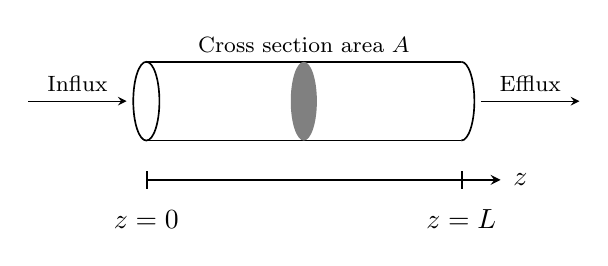
\begin{tikzpicture}[>=stealth]
			\draw[semithick] (0,0) -- (4,0);% bottom line
			\draw[semithick] (0,1) -- (4,1);% top line
			\draw[semithick] (0,0.5) ellipse (0.166 and 0.5);% left ellipse
			\draw[semithick] (4,0) arc (-90:90:0.166 and 0.5);% right half of the right ellipse
			\draw[|-,semithick] (0,-0.5) -- (4,-0.5);
			\draw[|->,semithick] (4,-0.5) -- (4.5,-0.5);
			\draw (0,-1) node {$z=0$};
			\draw (4,-1) node {$z=L$};
			\node at (4.75, -0.5) {$z$};

			\draw[->] (-1.5,0.5) -- (-0.25,0.5) node[above,midway,sloped,font=\footnotesize] {Influx};
			\draw[->] (4.25,0.5) -- (5.5,0.5) node[above,midway,sloped,font=\footnotesize] {Efflux};

			\fill[gray] (2,0.5) ellipse (0.166 and 0.5);
			\node[above,font=\footnotesize] at (2,1) {Cross section area $A$};
		\end{tikzpicture}
	}
	\subcaptionbox{A section of the column\label{fig:ModelGRMColumnSection}}[0.48 \linewidth]{%
		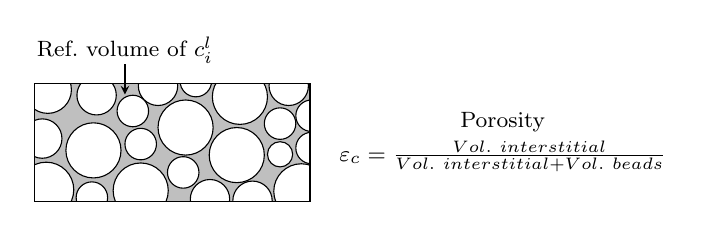
\begin{tikzpicture}[>=stealth]
			\begin{scope}
				\clip (0.25,0.25) rectangle (3.75,1.75);
				\fill[semithick,color=black!25!white] (0.25,0.25) rectangle (3.75,1.75);
%				\draw[semithick] (0,0) rectangle (4,2);
				\filldraw[color=black,fill=white] (0.4,0.4) circle[radius=0.35cm];
				\filldraw[color=black,fill=white] (0.35,1.05) circle[radius=0.25cm];
				\filldraw[color=black,fill=white] (0.42,1.67) circle[radius=0.3cm];
				\filldraw[color=black,fill=white] (0.98,0.3) circle[radius=0.2cm];
				\filldraw[color=black,fill=white] (1,0.9) circle[radius=0.35cm];
				\filldraw[color=black,fill=white] (1.04,1.6) circle[radius=0.25cm];
				\filldraw[color=black,fill=white] (1.6,0.39) circle[radius=0.35cm];
				\filldraw[color=black,fill=white] (1.6,0.98) circle[radius=0.2cm];
				\filldraw[color=black,fill=white] (1.5,1.4) circle[radius=0.2cm];
				\filldraw[color=black,fill=white] (1.82,1.72) circle[radius=0.25cm];
				\filldraw[color=black,fill=white] (2.48,0.28) circle[radius=0.25cm];
				\filldraw[color=black,fill=white] (2.14,0.62) circle[radius=0.2cm];
				\filldraw[color=black,fill=white] (2.17,1.19) circle[radius=0.35cm];
				\filldraw[color=black,fill=white] (2.3,1.78) circle[radius=0.2cm];
				\filldraw[color=black,fill=white] (3.02,0.26) circle[radius=0.25cm];
				\filldraw[color=black,fill=white] (2.82,0.84) circle[radius=0.35cm];
				\filldraw[color=black,fill=white] (2.86,1.58) circle[radius=0.35cm];
				\filldraw[color=black,fill=white] (3.64,0.38) circle[radius=0.35cm];
				\filldraw[color=black,fill=white] (3.37,1.24) circle[radius=0.2cm];
				\filldraw[color=black,fill=white] (3.37,0.85) circle[radius=0.16cm];
				\filldraw[color=black,fill=white] (3.48,1.72) circle[radius=0.25cm];
				\filldraw[color=black,fill=white] (3.77,0.93) circle[radius=0.2cm];
				\filldraw[color=black,fill=white] (3.77,1.34) circle[radius=0.2cm];
			\end{scope}
			\draw[thin,color=black] (0.25,0.25) rectangle (3.75,1.75);

			\draw[<-] (1.4, 1.61) -- (1.4, 2);
			\node at (1.4, 2.17) {\footnotesize Ref.\ volume of $c^l_i$};
			\node[anchor=west,align=center] at (4,1) {\footnotesize Porosity\\ \footnotesize$\varepsilon_c = \frac{\text{Vol.~interstitial}}{\text{Vol.~interstitial} + \text{Vol.~beads}}$};
		\end{tikzpicture}
	}
	\caption{Column bulk model\label{fig:ModelGRMColumn}}
\end{figure}

The GRM describes transport of solute molecules through the interstitial column volume by convective flow, band broadening caused by axial dispersion, mass transfer resistance through a stagnant film around the beads, pore (and surface) diffusion in the porous beads \cite{Ma1996, Schneider1968a, Miyabe2007}, and adsorption to the inner bead surfaces.

Consider a column of length $L>0$ filled with spherical beads of (possibly) multiple types with radius $r_{p,j} \ll L$ (see Fig.~\ref{fig:ModelGRMColumn}), where $j$ is the particle type index. 
The mass balance in the interstitial column volume is described by
\begin{align}
	\frac{\partial c^l_i}{\partial t} &= -u \frac{\partial c^l_i}{\partial z} + D_{\text{ax},i} \frac{\partial^2 c^l_i}{\partial z^2} - \frac{1}{\beta_c} \sum_j d_j \frac{3}{r_{p,j}} k_{f,j,i} \left[ c^l_i - c^p_{j,i}(\cdot, \cdot, r_{p,j}) \right] + f_{\text{react},i}^l\left(c^l\right). \label{eq:ModelColumn}
\end{align}
Here, $c^l_i\colon \left[0, T_{\text{end}}\right] \times [0, L] \rightarrow \mathds{R}^{\geq 0}$ denotes the concentration in the interstitial column volume, $c^p_{j,i}\colon \left[0, T_{\text{end}}\right] \times [0, L] \times [r_{c,j}, r_{p,j}] \rightarrow \mathds{R}^{\geq 0}$ the liquid phase concentration in the beads, $k_{f,j,i}$ the film diffusion coefficient, $D_{\text{ax},i}$ the dispersion coefficient, $u$ the interstitial velocity, $d_j$ the volume fraction of particle type $j$, and $\beta_c = \varepsilon_c / (1 - \varepsilon_c)$ the column phase ratio, where $\varepsilon_c$ is the column porosity (ratio of interstitial volume to total column volume).
If reactions are considered, the term $f_{\text{react},i}^l\left(c^l\right)$ represents the net change of concentration $c_i$ due to reactions involving component $i$.

Danckwerts boundary conditions \cite{Danckwerts1953} are applied to inlet and outlet of the column:
\begin{align}
	u c_{\text{in},i}(t) &= u c^l_i(t,0) - D_{\text{ax},i} \frac{\partial c^l_i}{\partial z}(t, 0) \label{eq:BCInlet} & \forall t > 0,\\
	\frac{\partial c^l_i}{\partial z}(t, L) &= 0 & \forall t > 0. \label{eq:BCOutlet}
\end{align}
Note that the outlet boundary condition Eq.~\eqref{eq:BCOutlet} is also known as ``do nothing'' or natural outflow condition.

In the liquid phase of the porous beads (see Fig.~\ref{fig:ModelGRMBead}) the mass balance is given by
\begin{equation} \begin{split}
	\frac{\partial c^p_{j,i}}{\partial t} + \frac{1 - \varepsilon_{p,j}}{F_{\text{acc},j,i} \varepsilon_{p,j}} \frac{\partial}{\partial t} \sum_{m_{j,i}} c^s_{j,i,m_{j,i}} = &\underbrace{D_{p,j,i} \left[\frac{\partial^2}{\partial r^2} + \frac{2}{r} \frac{\partial}{\partial r} \right]c^p_{j,i}}_{\text{Pore diffusion}} \\
	&+ \underbrace{\frac{1 - \varepsilon_{p,j}}{F_{\text{acc},j,i} \varepsilon_{p,j}} D_{s,j,i} \left[\frac{\partial^2}{\partial r^2} + \frac{2}{r} \frac{\partial }{\partial r} \right] \sum_{m_{j,i}} c^s_{j,i,m_{j,i}} }_{\text{Surface diffusion}} \\
	&+ f_{\text{react},j,i}^p\left( c_j^p, c_j^s \right) + \frac{1 - \varepsilon_{p,j}}{F_{\text{acc},j,i} \varepsilon_{p,j}} f_{\text{react},j,i}^s\left( c_j^p, c_j^s \right), \label{eq:ModelBead}
\end{split}\end{equation}
where $c^s_{j,i,m_{j,i}}\colon \left[0, T_{\text{end}}\right] \times [0,L] \times [r_{c,j}, r_{p,j}] \rightarrow \mathds{R}^{\geq 0}$ denotes the solid phase concentration of the $i$th component's $m_{j,i}$th bound state in the beads of $j$th type, $D_{p,j,i}$ the effective diffusion coefficient in the beads, $D_{s,j,i}$ the surface diffusion coefficient, $F_{\text{acc},j,i} \in [0,1]$ the pore accessibility factor, and $\varepsilon_{p,j}$ the particle porosity (ratio of pore volume to total bead volume).
The inner bead radius $r_{c,j} \in [0, r_{p,j})$ is assumed to be $0$ by default, but can be positive in order to account for core-shell particles that have an impermeable core.
Reaction terms in liquid and solid phase are collected in $f_{\text{react},j,i}^p( c_j^p, c_j^s)$ and $f_{\text{react},j,i}^s(c_j^p, c_j^s)$, respectively.

The GRM is used with both quasi-stationary (Eq.~\eqref{eq:REqBinding}) and dynamic (Eq.~\eqref{eq:DynBinding}) binding models. \index{Binding!Models}\index{Binding!Dynamic}\index{Binding!Quasi-stationary}
\begin{alignat}{2}
	\text{quasi-stationary: }& & 0 &= f_{\text{ads},j}\left( c^p_j, c^s_j\right), \label{eq:REqBinding} \\
	\text{dynamic: }& & \frac{\partial c^s_j}{\partial t} &= D_{s,j} \left[\frac{\partial^2}{\partial r^2} + \frac{2}{r} \frac{\partial }{\partial r} \right] c^s_{j} + f_{\text{ads},j}\left( c^p_j, c^s_j\right) + f_{\text{react},j}^s\left( c_j^p, c_j^s \right). \label{eq:DynBinding}
\end{alignat}
Note that $c^p_j$ and $c^s_j$ denote the vector of all $c^p_{j,i}$ and $c^s_{j,i,m_{j,i}}$, respectively.

The boundary conditions of the bead model the film diffusion and are given for all ${t \in (0,\infty)}$ and $z \in [0,L]$ by
\begin{align}
	k_{f,j,i}\left[ c^l_i - c^p_{j,i}(\cdot, \cdot, r_{p,j}) \right] &= F_{\text{acc},j,i} \varepsilon_{p,j} D_{p,j,i} \frac{\partial c^p_{j,i}}{\partial r}(\cdot, \cdot, r_{p,j}) + \left( 1 - \varepsilon_{p,j}\right) D_{s,j,i} \sum_{m_{j,i}} \frac{\partial c^s_{j,i,m_{j,i}}}{\partial r}(\cdot, \cdot, r_{p,j}), \label{eq:BCBeadIn} \\
	\frac{\partial c^p_{j,i}}{\partial r}(\cdot, \cdot, r_{c,j}) &= 0. \label{eq:BCBeadCenter}
\end{align}
By default, the following initial conditions are applied for all $z \in [0,L]$ and $r \in \left[r_{c,j}, r_{p,j}\right]$:
\begin{align}
	c^l_i(0, z) &= 0, & c^p_{j,i}(0, z, r) &= 0, & c^s_{j,i,m_{j,i}}(0,z,r) &= 0. \label{eq:InitialConditions}
\end{align}

\begin{figure}[!hptb]
	\centering
	\subcaptionbox{Mass transport into beads\label{fig:ModelGRMBeadTransport}}[0.38 \linewidth]{%
		\begin{tikzpicture}[>=stealth]

			\fill[line width=2pt,color=black!25!white] ($(-35:2cm) + (-1,0)$) -- (-35:2cm) arc[start angle=-35,end angle=35,radius=2] -- +(-1,0) -- cycle;
			\draw[line width=0.15cm,color=black!45!white] (-35:2.075cm) arc[start angle=-35,end angle=35,radius=2.075];

			\draw[semithick] (-35:2cm) arc[start angle=-35,end angle=-10,radius=2];
			\draw[semithick] (10:2cm) arc[start angle=10,end angle=35,radius=2];
			\fill[semithick,white] ($(-1.35,0)+(-10:2cm)$) -- (-10:2cm) arc[start angle=-10,end angle=10,radius=2] -- +(-1.35,0) -- cycle;

			\node[anchor=east] at (1.65,0.75) {\footnotesize Bead};

			\node[anchor=east] at (0.5, -0) {\footnotesize $c^p_{i}$};
			\node[anchor=west] at (2.5, -0) {\footnotesize $c^l_{i}$};

			% Channel
			\filldraw[blue] (1,0) circle (0.08cm);
			\filldraw[blue] (1.3,0.01) circle (0.08cm);
			\filldraw[blue] (1.5,0.1) circle (0.08cm);
			\filldraw[blue] (1.2,0.23) circle (0.08cm);
			\filldraw[blue] (1.13,-0.21) circle (0.08cm);
			\filldraw[blue] (0.9,0.18) circle (0.08cm);
			\filldraw[blue] (0.8,-0.25) circle (0.08cm);
			\filldraw[blue] (1.47,-0.22) circle (0.08cm);
			\filldraw[blue] (1.59,-0.05) circle (0.08cm);
			\filldraw[blue] (1.64,0.24) circle (0.08cm);
			\filldraw[blue] (1.79,-0.19) circle (0.08cm);
			\filldraw[blue] (1.79,0) circle (0.08cm);
			\filldraw[blue] (1.84,0.2) circle (0.08cm);

			% Outside
			\filldraw[blue] (2.27,-0.39) circle (0.08cm);
			\filldraw[blue] (2.25,-0.2) circle (0.08cm);
			\filldraw[blue] (2.4,0.02) circle (0.08cm);
			\filldraw[blue] (2.3,0.18) circle (0.08cm);
			\filldraw[blue] (2.34,0.36) circle (0.08cm);
			\filldraw[blue] (2.14,0.73) circle (0.08cm);
			\filldraw[blue] (2.19,0.52) circle (0.08cm);
			\filldraw[blue] (2.13,-0.79) circle (0.08cm);
			\filldraw[blue] (2.17,-0.58) circle (0.08cm);
			\filldraw[blue] (2.07,0.93) circle (0.08cm);
			\filldraw[blue] (2,1.1) circle (0.08cm);
			\filldraw[blue] (2.04,-0.97) circle (0.08cm);
			\filldraw[blue] (1.95,-1.15) circle (0.08cm);

			\begin{scope}[rotate=-2,xshift=0.32cm,yshift=-0.10cm]
				\filldraw[blue] (2.14,0.75) circle (0.08cm);
				\filldraw[blue] (2.19,0.51) circle (0.08cm);
				\filldraw[blue] (2.07,1.01) circle (0.08cm);
				\filldraw[blue] (2,1.21) circle (0.08cm);
			\end{scope}

			\begin{scope}[rotate=5,xshift=0.32cm,yshift=0.14cm]
				\filldraw[blue] (2.13,-0.73) circle (0.08cm);
				\filldraw[blue] (2.17,-0.56) circle (0.08cm);
				\filldraw[blue] (2.04,-0.97) circle (0.08cm);
				\filldraw[blue] (1.95,-1.19) circle (0.08cm);
			\end{scope}

			\draw[semithick,<->] (1.88,0) -- (2.28,0);
		\end{tikzpicture}
	}
	\subcaptionbox{Mass transport inside bead\label{fig:ModelGRMBeadDiff}}[0.58 \linewidth]{%
		\begin{tikzpicture}[>=stealth]

			\fill[semithick,fill=black!25!white] (0,0) circle (1);

			\draw[semithick] (0,0)+(xyz polar cs:angle=35,radius=1) arc[start angle=35,end angle=115,radius=1];
			\draw[semithick] (0,0)+(xyz polar cs:angle=125,radius=1) arc[start angle=125,end angle=215,radius=1];
			\draw[semithick] (0,0)+(xyz polar cs:angle=225,radius=1) arc[start angle=225,end angle=285,radius=1];
			\draw[semithick] (0,0)+(xyz polar cs:angle=295,radius=1) arc[start angle=295,end angle=385,radius=1];

			\draw[color=white,line width=5pt,line cap=round,line join=round] (xyz polar cs:angle=30,radius=1) .. controls (xyz polar cs:angle=30,radius=0.9) and (xyz polar cs:angle=55,radius=0.7) .. (0.2,0.1);
			\draw[color=white,line width=5pt,line cap=round,line join=round] (xyz polar cs:angle=120,radius=1) .. controls (xyz polar cs:angle=120,radius=0.9) and (xyz polar cs:angle=55,radius=0.7) .. (0.3,0.3);

			\draw[color=white,line width=3pt,line cap=round,line join=round] (0.1,0.5) .. controls (-0.2,0.3) .. (-0.3,0.3);
			\draw[color=white,line width=3pt,line cap=round,line join=round] (-0.2,0.3) .. controls (-0.2,0.3) .. (0.2,0.15);

			\draw[color=white,line width=5pt,line cap=round,line join=round] (xyz polar cs:angle=220,radius=1) .. controls (xyz polar cs:angle=220,radius=0.98) and (xyz polar cs:angle=205,radius=0.7) .. (0.3,-0.3) .. controls (0.2,-0.4) and (0.5,0) .. (0.7,0);
			\draw[color=white,line width=5pt,line cap=round,line join=round] (xyz polar cs:angle=290,radius=1) .. controls (xyz polar cs:angle=290,radius=0.98) and (xyz polar cs:angle=330,radius=0.7) .. (-0.5,0.4);

			\draw[color=white,line width=3pt,line cap=round,line join=round] (-0.2,0.1) .. controls (-0.5,-0.3) and (-0.4, -0.3) .. (-0.5,-0.4);
			\draw[color=white,line width=3pt,line cap=round,line join=round] (-0.7,-0.55) .. controls (-0.6,-0.75) and (-0.15,-0.8) .. (-0.1,-0.7);
			\draw[color=white,line width=3pt,line cap=round,line join=round] (-0.4,0.35) .. controls (-0.4,0.15) and (-0.9,0.1) .. (-0.8,-0.1);

			\draw[line width=0.1cm,color=black!45!white] (0,0) circle (1.051);

			\draw[<->] (xyz polar cs:angle=117.5,radius=0.85) -- (xyz polar cs:angle=120,radius=1.3) node[pos=0.5,xshift=-0.05cm] (FD) {};
			\node[anchor=south east,inner sep=1pt] (FDdesc) at (-1.2,1.2) {\footnotesize Film diffusion};
			\draw[very thin] (FD.center) -- (FDdesc);

			\draw[<->] (0,0.82) -- (0.3,0.66) node[midway,xshift=0.05cm,yshift=0.05cm] (SD) {};
			\node[anchor=south west,right=1.8cm of FDdesc,inner sep=1pt] (SDdesc) {\footnotesize Surface diffusion};
			\draw[very thin] (SD.center) -- (SDdesc);

			\draw[<->] (-0.60,-0.52) -- (-0.72,-0.28) node[midway,xshift=-0.05cm,yshift=-0.025cm] (S) {};
			\node[anchor=base east,inner sep=1pt] (Sdesc) at (-1.2,-0.9) {\footnotesize Adsorption};
			\draw[very thin] (S.center) -- (Sdesc);

			\draw[<->] (xyz polar cs:angle=297,radius=0.85) -- (xyz polar cs:angle=305,radius=0.4) node[pos=0.5,xshift=0.05cm] (PD) {};
			\node[anchor=base west,right=2.4cm of Sdesc,inner sep=1pt] (PDdesc)  {\footnotesize Pore diffusion\vphantom{p}};
			\draw[very thin] (PD.center) -- (PDdesc);

			\draw[<-] (-0.6,0.62) -- (-1.2,0.62);
			\node[anchor=east] at (-1.2,0.62) {\footnotesize Ref. volume of $c^s_{j,i,m_{j,i}}$};

			\draw[<-] (-0.8,0) -- (-1.2,0);
			\node[anchor=east] at (-1.2,0) {\footnotesize Ref. volume of $c^p_{j,i}$};

			\node[anchor=west,align=center] at (1.5,0.2) {\footnotesize Porosity\\ \footnotesize$\varepsilon_{p,j} = \frac{\text{Vol.~channels}}{\text{Vol.~channels} + \text{Vol.~solid}}$};

%			\draw[step=0.1cm,gray,thin] (-1,-1) grid (1,1);
		\end{tikzpicture}
	}
	\caption{Column bead model\label{fig:ModelGRMBead}}
\end{figure}


\begin{figure}[!hptb]
	\centering
	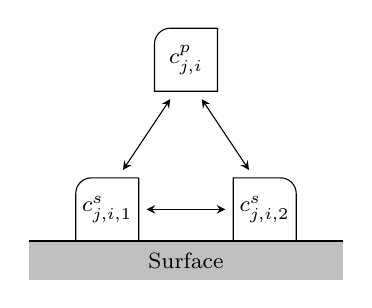
\begin{tikzpicture}[>=stealth]

		\fill[fill=black!25!white] (-0.5,0) rectangle (3.5,0.5);
		\draw[semithick] (-0.5,0.5) -- (3.5,0.5);.

		\begin{scope}[xshift=1.5cm,yshift=2.8cm]
%			\draw (0.2,0.2) -- (0,0.2) -- (-0.2,0) -- (-0.2,-0.2) -- (0.2,-0.2) -- (0.2,0.2);
%			\draw (0.4,0.2) -- (-0.2,0.2)  arc[radius=0.2cm,start angle=90,end angle=180] -- (-0.4,-0.2) -- (0.4,-0.2) -- (0.4,0.2);
			\draw (0.4,0.4) -- (-0.2,0.4)  arc[radius=0.2cm,start angle=90,end angle=180] -- (-0.4,-0.4) -- (0.4,-0.4) -- (0.4,0.4);
			\node at (0,0) {\footnotesize $c^p_{j,i}$};
		\end{scope}

		\begin{scope}[xshift=0.5cm,yshift=0.9cm]
			\draw (0.4,0.4) -- (-0.2,0.4)  arc[radius=0.2cm,start angle=90,end angle=180] -- (-0.4,-0.4) -- (0.4,-0.4) -- (0.4,0.4);
			\node at (0,0) {\footnotesize $c^s_{j,i,1}$};
		\end{scope}

		\begin{scope}[xshift=2.5cm,yshift=0.9cm,rotate=-90]
			\draw (0.4,0.4) -- (-0.2,0.4)  arc[radius=0.2cm,start angle=90,end angle=180] -- (-0.4,-0.4) -- (0.4,-0.4) -- (0.4,0.4);
			\node at (0,0) {\footnotesize $c^s_{j,i,2}$};
		\end{scope}

		\node at (1.5, 0.25) {\footnotesize Surface};

		\draw[<->] (0.7,1.4) -- (1.3,2.3);
		\draw[<->] (2.3,1.4) -- (1.7,2.3);
		\draw[<->] (1,0.9) -- (2,0.9);
	\end{tikzpicture}
	\caption{Binding with multiple bound states}
\end{figure}

See Table~\ref{tab:FFModelUnitOpGRM}.

\paragraph{Particle geometry}
\phantomsection\label{par:MUOPGRMParticleGeometry}

In the model above, spherical particles are considered.
Other supported particle forms are cylinders and slabs.
For cylinders, it is assumed that molecules can only enter through the lateral surface (i.e., the caps are sealed).
Slabs are assumed to have two large sides such that molecules enter through the two large faces (i.e., the remaining four small faces are sealed).

All particle forms support core-shell beads that have an impermeable core.
The particles are characterized by their (outer) ``radius'' $r_{p,j}$ and their (inner) core ``radius'' $r_{c,j} \in [0, r_{p,j})$.
See Fig.~\ref{fig:ModelGRMParticleGeometries}.

\begin{figure}[!hptb]
	\centering
	\begin{tikzpicture}[>=stealth]

		\draw (0,0) circle (2cm);
		\draw[dashed] (2,0) arc (0:180:2 and 0.6);
		\path[fill=white,draw=black] (0,0) circle (0.75cm);
		\draw[dashed] (0.75,0) arc (0:180:0.75 and 0.225);
		\draw (-0.75,0) arc (180:360:0.75 and 0.225);

		\draw (-2,0) arc (180:360:2 and 0.6);

		\fill[fill=black] (0,0) circle (1pt);
		\draw[dashed] (0,0 ) -- node[above]{$r_{c}$} (2,0);
		\node[right] at (2,0) {$r_p$};

		\begin{scope}[shift={(4.5,0)}]
			\node[cylinder,draw=black,aspect=3.25,minimum height=3.5cm,minimum width=2.5cm,shape border rotate=0,] (column) {};
			%cylinder uses custom fill, cylinder body fill=red!30,cylinder end fill=red!10

			\draw[dashed]
				let \p1 = ($ (column.after bottom) - (column.before bottom) $),
					\n1 = {0.5*veclen(\x1,\y1)-0.5\pgflinewidth},
					\p2 = ($ (column.bottom) - (column.after bottom)!.5!(column.before bottom) $),
					\n2 = {veclen(\x2,\y2)-0.5\pgflinewidth}
				in
					([yshift=-0.5\pgflinewidth] column.before bottom) arc [start angle=-90, end angle=90, y radius=\n1, x radius=\n2];

			\draw[]
				let \p1 = ($ (column.before top) - (column.after top) $),
					\n1 = {0.4*(0.5*veclen(\x1,\y1)-0.5\pgflinewidth)},
					\p2 = ($ (column.top) - (column.before top)!.5!(column.after top) $),
					\n2 = {0.4*(veclen(\x2,\y2)-0.5\pgflinewidth)}
				in
					([yshift=-0.75cm] column.before top) arc [start angle=90, end angle=-270, y radius=\n1, x radius=\n2];

			\draw[dashed]
				let \p1 = ($ (column.before top) - (column.after top) $),
					\n1 = {0.4*(0.5*veclen(\x1,\y1)-0.5\pgflinewidth)},
					\p2 = ($ (column.top) - (column.before top)!.5!(column.after top) $),
					\n2 = {0.4*(veclen(\x2,\y2)-0.5\pgflinewidth)}
				in
					([yshift=-0.75cm] column.after bottom) arc [start angle=90, end angle=-270, y radius=\n1, x radius=\n2];

			\draw[dashed] ([yshift=-0.75cm] column.after bottom) -- ([yshift=-0.75cm] column.before top);
			\draw[dashed] ([yshift=0.75cm] column.before bottom) -- ([yshift=0.75cm] column.after top);
		
			\fill[fill=black] (0,0) circle (1pt);
			\draw[dashed] (0,0) -- (0,1.25) node[above] {$r_p$};
			\node[above,right] at (0,0.75) {$r_c$};
		\end{scope}

		\begin{scope}[shift={(9,-0.5)}]
		
			\draw (-1.5,-0.125) rectangle (1.5,0.125);
			\draw (-1.5,0.125) rectangle (1.5,0.5);
			\draw (-1.5,-0.125) rectangle (1.5,-0.5);

			\draw (-1.5,0.5) -- ++(1.35,1.2) -- ++(3,0) -- ++(-1.35,-1.2);
			\draw[dashed] (-1.5,-0.5) -- ++(1.35,1.2) -- ++(3,0);
			\draw (2.85,1.7) -- ++(0,-1) -- (1.5,-0.5);
			\draw[dashed] (-0.15,1.7) -- ++(0,-1);

			\draw[dashed] (-1.5,-0.125) -- ++(1.35,1.2) -- ++(3,0); % -- ++(-1.35,-1.2);
			\draw (1.5,-0.125) -- ++(1.35,1.2);
			\draw[dashed] (-1.5,0.125) -- ++(1.35,1.2) -- ++(3,0); % -- ++(-1.35,-1.2);
			\draw (1.5,0.125) -- ++(1.35,1.2);

			\fill[fill=black] (0,0) circle (1pt);
			\draw[dashed] (0,0) -- (0,-0.5) node[below] {$r_p$};
			\node[below,right] at (0,-0.125) {$r_c$};

		\end{scope}

	\end{tikzpicture}
	\caption{Particle geometries\label{fig:ModelGRMParticleGeometries}}
\end{figure}

For cylinders, the factor $3 / r_{p,j}$ in \eqref{eq:ModelColumn} changes to $2 / r_{p,j}$ and the diffusion operator in \eqref{eq:ModelBead} and \eqref{eq:DynBinding} changes as
\begin{align*}
	\left[\frac{\partial^2}{\partial r^2} + \frac{2}{r} \frac{\partial }{\partial r} \right] \quad \rightarrow \quad \left[\frac{\partial^2}{\partial r^2} + \frac{1}{r} \frac{\partial }{\partial r} \right].
\end{align*}
For slabs, the factor $3 / r_{p,j}$ in \eqref{eq:ModelColumn} changes to $1 / r_{p,j}$ and the diffusion operator in \eqref{eq:ModelBead} and \eqref{eq:DynBinding} changes as
\begin{align*}
	\left[\frac{\partial^2}{\partial r^2} + \frac{2}{r} \frac{\partial }{\partial r} \right] \quad \rightarrow \quad \frac{\partial^2}{\partial r^2}.
\end{align*}

\paragraph{Multiple particle types}
\phantomsection\label{par:MUOPGRMMultiParticleTypes}

A particle type \index{Model!Multiple particle types}\index{Model!Particle types} has its own set of mass transfer and geometry parameters $\varepsilon_{p,j}$, $D_{p,j}$, $D_{s,j}$, etc.\ (see Eq.~\eqref{eq:ModelBead}) and its own binding model $f_{\mathrm{ads}}$ (including a possibly differing number of bound states).
This allows, for example, modeling of particle size distributions or potential applications with differently functionalized beads (e.g., immobilized enzymes).

The distribution of the particle types is governed by their volume fractions $d_j$ in Eq.~\eqref{eq:ModelColumn}.
The volume fractions have to sum to $1$:
\begin{align*}
	\sum_{j=0}^{N_{\text{partype}} - 1} d_j = 1.
\end{align*}

The particle type volume fractions can be spatially constant throughout the column, or depend on the position inside the column bulk volume.
In the latter case, the user can specify a set of volume fractions for each discretized finite volume cell.
This allows, for example, the placement of smaller particles near the frits.

\paragraph{Size exclusion chromatography}
\phantomsection\label{par:MUOPGRMSizeExclusion}

The general rate model can be used to simulate size exclusion chromatography (SEC) \cite{Gu1995}. \index{Model!Size exclusion chromatography}
The particle porosity $\varepsilon_{p,j}$ on the mobile phase side of the transport equations is replaced by a component-dependent accessible porosity
\begin{align}
	\varepsilon_{p,j,i} = F_{\text{acc},j,i} \varepsilon_{p,j},
\end{align}
where the pore accessibility factor $F_{\text{acc},j,i}$ ranges in $(0, 1]$.

Small molecules that can enter any pore have $F_{\text{acc},j,i} = 1$, whereas larger molecules that can enter some, but not small pores, have values $0 < F_{\text{acc},j,i} < 1$.
The other extreme is given by molecules so large that they cannot enter any pore and, consequently, $F_{\text{acc},j,i} = 0$.
Note that $F_{\text{acc},j,i} = 0$ is not allowed in a simulation, which can be circumvented by setting $k_{f,j,i} = 0$.

By default, $F_{\text{acc},j,i} = 1$ for all components $i$ and all particle types $j$, which disables size exclusion chromatography.
In order to simulate pure SEC, binding is disabled by setting $N_{\text{bnd},i} = 0$ for all components $i$ and applying no binding model.
If adsorption is present, it is important to note that any saturation capacity (e.g., $q_{\text{max}}$ of Langmuir-type binding models) is subject to the full pore volume fraction $\varepsilon_{p,j}$.

Note that multiple particle types can also be used to aid in modeling size exclusion effects, see~Section~\ref{par:MUOPGRMMultiParticleTypes}.

\paragraph{Specification of flow rate / velocity and direction}
\phantomsection\label{par:MUOPGRMflow}

Since volumetric flow rates are specified for each network connection, the unit operation can infer its interstitial velocity via
\begin{align*}
	u = u_{\text{int}} = \frac{F_{\text{in}}}{A \varepsilon_c},
\end{align*}
where $F_{\text{in}}$ denotes the volumetric flow rate and $A$ the cross section area.
Note that without the bulk porosity $\varepsilon_c$, the superficial velocity would be obtained.

The direction of flow inside the unit operation is governed by the sign of the interstitial velocity $u$.
A positive sign results in (standard) forward flow, whereas a negative sign reverses the flow direction.
Note that in case of reversed flow, the chromatogram is returned at the unit operation's \emph{inlet}, which may not be returned from simulation by default.

The final behavior is controlled by the interplay of cross section area and interstitial velocity:
\begin{enumerate}
	\item If cross section area $A$ is given and $u$ is not, $u$ is inferred from the volumetric flow rate.
	\item If $u$ is given and $A$ is not, the volumetric flow rate is ignored and the provided interstitial velocity is used.
	\item If both cross section area $A$ and interstitial velocity $u$ are given, the magnitude of the actual interstitial velocity $u$ is inferred from the volumetric flow rate and the flow direction is given by the sign of the provided $u$.
\end{enumerate}

\subsection{Lumped rate model with pores (LRMP)}\label{sec:MUOPLRMP}

The lumped rate model with pores \index{Model!Lumped rate model with pores}\index{Model!LRMP}\index{Unit operation!Lumped rate model with pores}\index{Unit operation!LRMP} \cite{Guiochon2006,Felinger2004} deviates from the general rate model (see Section~\ref{sec:MUOPGRM}) by neglecting pore diffusion.
The particle phase $c^p_j$ is still there, but no mass transfer happens except for binding and film diffusion.
Hence, the model equations are given by
\begin{align}
	\frac{\partial c^l_i}{\partial t} &= -u \frac{\partial c^l_i}{\partial z} + D_{\text{ax},i} \frac{\partial^2 c^l_i}{\partial z^2} - \frac{1}{\beta_c} \sum_{j} d_j \frac{3}{r_{p,j}} k_{f,j,i}\left[ c^l_i - c^p_{j,i} \right] + f_{\text{react},i}^l\left(c^l\right), \\
	\begin{split}
	\frac{\partial c^p_{j,i}}{\partial t} &+ \frac{1 - \varepsilon_{p,j}}{F_{\text{acc},j,i} \varepsilon_{p,j}} \frac{\partial}{\partial t} \sum_{m_{j,i}} c^s_{j,i,m_{j,i}} = \frac{3}{F_{\text{acc},j,i} \varepsilon_{p,j} r_{p,j}}k_{f,j,i}\left[ c^l_i - c^p_{j,i} \right] \\
	&\qquad\qquad\qquad\qquad\qquad\qquad\qquad+ f_{\text{react},j,i}^p\left( c_j^p, c_j^s \right) + \frac{1 - \varepsilon_{p,j}}{F_{\text{acc},j,i} \varepsilon_{p,j}} f_{\text{react},j,i}^s\left( c_j^p, c_j^s \right)
	\end{split}
\end{align}
with the same meanings of variables and parameters as in the general rate model. 
The equations are complemented by Danckwerts boundary conditions \cite{Danckwerts1953}
\begin{align*}
	u c_{\text{in},i}(t) &= u c^l_i(t,0) - D_{\text{ax},i} \frac{\partial c^l_i}{\partial z}(t, 0) & \forall t > 0,\\
	\frac{\partial c^l_i}{\partial z}(t, L) &= 0 & \forall t > 0.
\end{align*}

As for the general rate model, both quasi-stationary and dynamic binding models are supported:
\begin{alignat*}{2}
	\text{quasi-stationary: }& & 0 &= f_{\text{ads},j}\left( c^p_j, c^s_j\right), \\
	\text{dynamic: }& & \frac{\partial c^s_j}{\partial t} &= f_{\text{ads},j}\left( c^p_j, c^s_j\right) + f_{\text{react},j}^s\left( c_j^p, c_j^s \right).
\end{alignat*}
By default, the following initial conditions are applied for all $z \in [0,L]$:
\begin{align}
	c^l_i(0, z) &= 0, & c^p_{j,i}(0, z) &= 0, & c^s_{j,i,m_{j,i}}(0,z) &= 0.
\end{align}

Multiple particle types and all particle geometries are supported (see Section~\ref{par:MUOPGRMMultiParticleTypes}).
This model can also be used to simulate size exclusion chromatography (see Section~\ref{par:MUOPGRMSizeExclusion}).\index{Model!Size exclusion chromatography}
For the specification of flow rate and direction, the same holds as for the general rate model (see Section~\ref{par:MUOPGRMflow}).
See Table~\ref{tab:FFModelUnitOpLRMP}.

\subsection{Lumped rate model without pores (LRM)}\label{sec:MUOPLRM}

The lumped rate model without pores \index{Model!Lumped rate model without pores}\index{Model!LRM}\index{Unit operation!Lumped rate model without pores}\index{Unit operation!LRM} \cite{Guiochon2006,Felinger2004} deviates from the lumped rate model with pores (see Section~\ref{sec:MUOPLRMP}) by neglecting pores completely.
The particle phase $c^p$ is removed and the porosity $\varepsilon_t$ is taken as total porosity
\begin{align}
	\varepsilon_t = \varepsilon_c + \left( 1 - \varepsilon_c \right) \varepsilon_p. \label{eq:TotalPorosity}
\end{align}
The phase ratio is denoted by $\beta_t = \varepsilon_t / (1 - \varepsilon_t)$ accordingly.
The model equations are given by
\begin{align}
	\frac{\partial c^l_i}{\partial t} + \frac{1}{\beta_t} \frac{\partial}{\partial t} \sum_{m_i} c^s_{i,m_i} &= -u \frac{\partial c^l_i}{\partial z} + D_{\text{ax},i} \frac{\partial^2 c^l_i}{\partial z^2} + f_{\text{react},i}^l\left( c^l, c^s \right) + \frac{1}{\beta_t} f_{\text{react},i}^s\left( c^l, c^s \right),
\end{align}
where $\beta_t = \varepsilon_t / (1 - \varepsilon_t)$ denotes the (total) phase ratio.
The equations are complemented by Danckwerts boundary conditions \cite{Danckwerts1953}
\begin{align*}
	u c_{\text{in},i}(t) &= u c^l_i(t,0) - D_{\text{ax},i} \frac{\partial c^l_i}{\partial z}(t, 0) & \forall t > 0,\\
	\frac{\partial c^l_i}{\partial z}(t, L) &= 0 & \forall t > 0.
\end{align*}

Both quasi-stationary and dynamic binding models are supported:
\begin{alignat*}{2}
	\text{quasi-stationary: }& & 0 &= f_{\text{ads}}\left( c^l, c^s\right), \\
	\text{dynamic: }& & \frac{\partial q}{\partial t} &= f_{\text{ads}}\left( c^l, c^s\right) + f_{\text{react}}^s\left( c^l, c^s \right).
\end{alignat*}
By default, the following initial conditions are applied for all $z \in [0,L]$:
\begin{align}
	c^l_i(0, z) &= 0, & c^s_{i,m_i}(0,z) &= 0.
\end{align}

Note that by setting $\varepsilon_t = 1$, removing all bound states by setting $N_{\text{bnd},i} = 0$ for all components $i$, and applying no binding model, a dispersive plug flow reactor (DPFR)\index{Model!Dispersive plug flow reactor}\index{Model!DPFR}\index{Unit operation!Dispersive plug flow reactor}\index{Unit operation!DPFR} is obtained.

For the specification of flow rate and direction, the same holds as for the general rate model (see Section~\ref{par:MUOPGRMflow}).
See Table~\ref{tab:FFModelUnitOpLRM}.

\subsection{Two Dimensional General rate model (GRM2D)}\label{sec:MUOPGRM2D}

The general rate model as introduced in Section~\ref{sec:MUOPGRM} assumes homogeneity in the cross sections of the column.
This allows to consider transport along the axial dimension only.
However, due to packing irregularity and inhomogeneous flow at the inlet (i.e., frits), this assumption may be a crude approximation.
This model can be improved by introducing a radial coordinate $\rho \in [0, R]$\index{Model!General rate model 2D}\index{Model!GRM 2D}\index{Unit operation!General rate model 2D}\index{Unit operation!GRM 2D}, where $R$ is the column radius, in the interstitial volume Eq.~\eqref{eq:ModelColumn}:
\begin{equation} \begin{split}
	\varepsilon_c \frac{\partial c^l_i}{\partial t} = &-\varepsilon_c u \frac{\partial c^l_i}{\partial z} + \varepsilon_c D_{\text{ax},i} \frac{\partial^2 c^l_i}{\partial z^2} + \frac{1}{\rho} \frac{\partial}{\partial \rho} \left( \rho D_{\text{rad},i} \frac{\partial}{\partial \rho} \left( \varepsilon_c c^l_i \right) \right) \\ &- \left(1 - \varepsilon_c\right) \sum_j d_j \frac{ 3 k_{f,j,i} }{r_{p,j}} \left[ c^l_i - c^p_{j,i}(\cdot, \cdot, \cdot, r_{p,j}) \right] + \varepsilon_c f_{\text{react},i}^l\left(c^l\right). \label{eq:ModelColumn2D}
\end{split} \end{equation}
Here, $c^l_i\colon \left[0, T_{\text{end}}\right] \times [0, L] \times [0, R] \rightarrow \mathds{R}^{\geq 0}$, $c^p_{j,i}\colon \left[0, T_{\text{end}}\right] \times [0, L] \times [0, R] \times [r_{c,j}, r_{p,j}] \rightarrow \mathds{R}^{\geq 0}$, and $c^s_{j,i,m_{j,i}}\colon \left[0, T_{\text{end}}\right] \times [0, L] \times [0, R] \times [r_{c,j}, r_{p,j}] \rightarrow \mathds{R}^{\geq 0}$ depend on $\rho$.
Additionally, the porosity $\varepsilon_c$, axial dispersion coefficient $D_{\text{ax},i}$, radial dispersion coefficient $D_{\text{rad},i}$, and interstitial velocity $u$ may depend on $\rho$.

The dependence of the parameters on $\rho$ is not arbitrary.
For simplicity, it is assumed that the parameters are piecewise constant, that is, the range $[0, R]$ is divided into disjoint zones in which all parameters are constant.
These zones are used for radial discretization and can be supplied to the simulator.
Continuous dependence of the parameters can be realized by piecewise constant approximation.

The Danckwerts boundary conditions at the column in- and outlet, Eq.~\eqref{eq:BCInlet} and \eqref{eq:BCOutlet}, are modified to account for the radial coordinate:
\begin{subequations}\label{eq:BCAxial2D}
\begin{align}
	u(\rho) c_{\text{in},i}(t,\rho) &= u(\rho) c^l_i(t,0,\rho) - D_{\text{ax},i}(\rho) \frac{\partial c^l_i}{\partial z}(t, 0, \rho) \label{eq:BCInlet2D} & \forall t > 0, \rho \in (0,R), \\
	\frac{\partial c^l_i}{\partial z}(t, L, \rho) &= 0 & \forall t > 0, \rho \in (0,R). \label{eq:BCOutlet2D}
\end{align}
\end{subequations}
Conditions for the radial direction are added:
\begin{subequations}\label{eq:BCRadial2D}
\begin{align}
	\frac{\partial{c^l_i}}{\partial \rho}(\cdot, \cdot, 0) &= 0, \label{eq:BCRadial2DInner} \\
	\frac{\partial{c^l_i}}{\partial \rho}(\cdot, \cdot, R) &= 0. \label{eq:BCRadial2DOuter}
\end{align}
\end{subequations}
While the inner condition Eq.\eqref{eq:BCRadial2DInner} represents symmetry at the column center, the outer condition Eq.~\eqref{eq:BCRadial2DOuter} is a no-flux condition.

Using the inlet boundary condition Eq.~\eqref{eq:BCInlet2D}, each radial zone is equipped with its own inlet and outlet port.
That is, this unit operation has as many inlet and outlet ports as it has radial zones (parameter \texttt{NRAD} in the \texttt{discretization} group).
This allows each radial zone to have its own inlet profile, which enables modeling of flow distribution in the frits by sending the feed through varying hold-up volumes before injecting it into a radial zone.

See Table~\ref{tab:FFModelUnitOpGRM2D}.

\paragraph{Specification of flow rate / velocity and direction}
\phantomsection\label{par:MUOPGRMflow2D}

Since the column radius $R$ and the zones $(\rho_k, \rho_{k+1})$, $k = 0, \dots, N_{\text{rad}} - 1$, are known, the interstitial velocities $u_k$ are inferred from the volumetric flow rates via
\begin{align*}
	u_k = u_{\text{int},k} = \frac{F_{\text{in},k}}{\pi \left( \rho_{k+1}^2 - \rho_k^2 \right) \varepsilon_{c,k}},
\end{align*}
where $F_{\text{in},k}$ denotes the volumetric flow rate into zone $k$.

The direction of flow inside the radial zone of the unit operation is governed by the sign of the interstitial velocity $u_k$.
A positive sign results in (standard) forward flow, whereas a negative sign reverses the flow direction.
Note that in case of reversed flow, the chromatogram is returned at the unit operation's \emph{inlet} port, which may not be returned from simulation by default.

Note that, contrary to the standard general rate model as presented in Section~\ref{sec:MUOPGRM}, the interstitial flow rate is always given by the volumetric flow rate.
The velocity parameter only determines the flow direction.

\subsection{Continuous stirred tank reactor model (CSTR)}\label{sec:MUOPCSTR}

The continuous stirred tank reactor model \index{Model!Continuous stirred tank reactor}\index{Model!CSTR}\index{Unit operation!Continuous stirred tank reactor model}\index{Unit operation!CSTR} is a basic building block in unit operation networks and often used to model holdup volume.
When combined with a binding model, it can be used to model batch uptake experiments.

Assuming that the fluid inside the tank is well-mixed and that the volume can vary, the governing equations are given by
\begin{align*}
	\frac{\mathrm{d}}{\mathrm{d}t} \left(\left[ c_i + \frac{1-\varepsilon}{\varepsilon} \sum_j d_j \sum_{m_{j,i}} c^s_{j,i,m_{j,i}} \right] V\right) &= F_{\text{in}} c_{\text{in},i} - F_{\text{out}} c_i + V f_{\text{react},i}^l\left( c \right) + V \frac{1-\varepsilon}{\varepsilon}\sum_j d_j f_{\text{react},j,i}^s\left( c, c_j^s \right),
\end{align*}
which balances the mass, the binding equation
\begin{alignat*}{2}
	\text{quasi-stationary: }& & 0 &= f_{\text{ads},j}\left( c, c^s_j\right), \\
	\text{dynamic: }& & \frac{\partial c^s_j}{\partial t} &= f_{\text{ads},j}\left( c, c^s_j\right) + f_{\text{react},j}^s\left( c, c_j^s \right),
\end{alignat*}
depending on whether quasi-stationary or dynamic binding is used, and the evolution of volume
\begin{align*}
	\frac{\mathrm{d}V}{\mathrm{d}t} &= F_{\text{in}} - F_{\text{out}} - F_{\text{filter}}.
\end{align*}
The porosity $\varepsilon$ denotes the ratio of liquid phase volume to total tank volume.
Thus, setting $\varepsilon = 1$, removing all bound states by setting $N_{\text{bnd},j,i} = 0$ for all components $i$ and particle types $j$, and applying no binding model results in a simple tank.
The additional parameter $F_{\text{filter}}$, which denotes the flow rate of pure liquid (without any components) out of the tank, can be used to model a filtering unit.

Note that it is the user's duty to make sure that the volume of the CSTR does not fall below \SI{0}{\cubic\metre}.
If it does, the simulation may fail to run or may produce unreasonable (e.g., unphysical) results.

See Table~\ref{tab:FFModelUnitOpCSTR}.
